\documentclass{article}

\usepackage[dutch]{babel}
\usepackage[version=3]{mhchem}
\usepackage{hyperref}
\usepackage{pdfpages}
\usepackage{graphicx}
\usepackage{marvosym}
\usepackage{graphicx}
\usepackage{wrapfig}
\usepackage{listings}
\usepackage[gen]{eurosym}

% Variables for source code colors
\definecolor{dkgreen}{rgb}{0,0.6,0}
\definecolor{gray}{rgb}{0.5,0.5,0.5}
\definecolor{mauve}{rgb}{0.58,0,0.82}

% Makeup for source code display
\lstset{
        language=C++,
        basicstyle={\small\ttfamily},
        numbers=left,
        numberstyle=\small\color{gray},
        numberstyle=\tiny\color{gray},
        keywordstyle=\color{blue},
        commentstyle=\color{dkgreen},
        stringstyle=\color{mauve},
	tabsize=2,
	breaklines=true,
}  
\usepackage{marvosym}
\usepackage{url} 

\begin{document}

\title{Documentatie Pinautomaat}
\author{Bytegroep 10}

\maketitle

\begin{abstract}

De opdracht voor dit project was om een werkende geldautomaat te maken.
In dit verslag zijn onderzoeksanalysen met adviezen terug te vinden.
Wij hebben aan de hand van deze adviezen hierna ontwerpen gemaakt en gerealizeerd.
Wij moeten tijdens de loop van het project letten op vijf onderdelen: \emph{beheren, analyseren, adviseren, ontwerpen en realiseren.}

\end{abstract}

\newpage

\tableofcontents

\newpage

\section{Beheren}

\subsection{Versiebeheer}

Voor dit onderdeel moesten wij kunnen werken met Git en Version control.
Hier is veel onderzoek over gedaan zodat het goed toegepast kan worden dit project.
In figuur \ref{fig: git model} is het model wat wij gebruiken op onze Git pagina, \href{https://github.com/Gewad/Project4Bankalicious}{Project4Bankalicious}.
Ieder groepslid werkt op zijn individuele branch, en als je klaar bent met jouw onderdeel, dan wordt hij in test gemerged.
Als er geen problemen lijken te zijn op de test beslissen wij in een groep of wij test naar de master kunnen schrijven.
Alle documentatie is terug te vinden op Github.

\begin{figure}[!h]
        \centering
        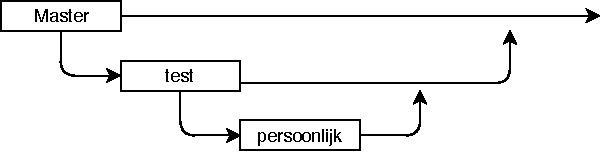
\includegraphics[height=0.7in]{git.pdf}
        \caption{git model}
        \label{fig: git model}
\end{figure}

\section{Samenwerkingscontract}

\paragraph{Financi\"en}

De kosten voor het gezamenlijke deel van de opdracht(en) worden gezamenlijk betaald, iedereen betaald even veel.

\paragraph{Schades}

Als er iets kapot gaat, worden de kosten van het vervangen gedeeld door de groep tenzij er opzettelijk of onverantwoordelijk mee om is gegaan.
In dat geval zullen de kosten voor de persoon die de schade heeft aangericht zijn.

\paragraph{Github afspraken}

\begin{itemize}
\item Niet op de master werken. Je werkt altijd op een eigen kopie van de test branch.
\item Gelieve geen word bestanden te uploaden zonder ook een pdf te uploaden.
\item Commits moeten duidelijk beschrijven wat er is aangepast. Liever een paar woorden teveel dan te weinig.
\item De repo van project 4 is geen zandbak om Git te testen.
\item Directories zijn met kleine letters en underscores, en hebben een duidelijke naam.
\item Alle benamingen en commits moeten in het Nederlands.
\item Branch namen zijn met kleine letters en woorden zijn verbonden met een min teken.
\end{itemize}

\paragraph{Te laat bij afspraken}

Al onze afspraken worden in goed overleg gepland daarom wordt er van groepsleden verwacht
dat ze op tijd zijn bij een afspraak (zowel deadlines als overleg) als een groepslid zonder goede
1
reden meer dan 5 minuten te laat is dan staat daar een consequentie tegen over. Deze
consequentie is of 20 chicken mcnuggets of een taart (let op: cake is geen taart!), als er
meerdere mensen te laat zijn moeten zij allebei iets mee nemen.

\paragraph{Afwezigheid bij afspraken}

Al onze afspraken worden in goed overleg gepland daarom wordt er van groepsleden verwacht
dat ze bij afspraken aanwezig zijn. als een groepslid zonder goede reden afwezig is bij een
overleg staat daar een consequentie tegenover. Deze consequentie is of 40 chicken mcnuggets
of twee taarten. Deze reden zal met de groep besproken moeten worden voordat het een geldige reden is.

\paragraph{Communicatie}

Communiceer goed, dat betekent duidelijk en met respect durf anderen aan te spreken.
Vraag hulp als je hulp nodig hebt.
Geef op tijd aan als je wil stoppen met de studie en draag alle onderdelen van het project tijdig
over aan een ander groepslid.

\paragraph{Rolverdeling}

De rolverdeling staat netjes gedocumenteerd op Github, en ieder teamlid is gediend deze zo
goed mogelijk uit te voeren.
\begin{itemize}
\item Paul H. Organizator
\item Paul W. Verbinder
\item Gerard Expert
\item Merijn Documentatie manager, onderzoeker
\item Aron Tester
\item Boas Kwaliteitsbewaker
\item Floor Designer, expert
\item Mohammed Designer
\end{itemize}

\newpage

\subsection{Kwaliteitseisen}

Aan het begin van het project hebben we een paar eisen besreven waar ons eindproduct aan moet voldoen, ze staan hieronder.

\subsubsection{Code eisen}
\begin{itemize}
\item De code moet leesbaar zijn voor iedereen dus ook voor mensen die het niet geschreven hebben. Het doel is dat al onze ouders ook kunnen begrijpen wat er staat, een onderdeel hier van is commends.
\item De code moet zo efficiënt mogelijk zijn.
Variabele moeten een goede en duidelijk naam hebben en een vaste structuur volgen, namen van klasse beginnen met een Hoofdletter, namen van andere variabelen beginnen met een kleine letter. 
	\item Als een variabele bestaat uit twee woorden begint het tweede woord met een Hoofdletter. Aka camelcase bv. camelCase.
	\item Splits zoveel mogelijk code op in classes en methodes. Stop bijbehorende code in een pakkage.
	\item Maak eerst een klasse diagram voor dat je gaat programmeren.
	\item In bestandsnamen mogen geen * worden gebruik dit vind Windows namelijk niet leuk.
\end{itemize}
\subsubsection{Product eisen}
\begin{itemize}
	\item De geldautomaat moet  biljetten van tenminste vier verschillende waarden uit kunnen geven
	\item De gebruiker kan niet, zonder een pin-opdracht te geven, geld uit de automaat halen
	\item De geldautomaat geeft altijd het juiste bedrag
	\item De geldautomaat geeft alleen geld als het saldo toereikend is
	\item De gebruiker kan zelf selecteren welke biljetten hij/zij wil ontvangen
	\item De gebruiker kan geen biljetten kiezen die niet aanwezig zijn in de geldautomaat
	\item De geldautomaat is robuust (kan zelfstandig staan en valt niet om/uit elkaar tijdens 	gebruik)
	\item De biljetten in de geldautomaat mogen maximaal de dikte van een speelkaart hebben
	\item Na het pinnen wordt er een bon geprint met een bonprinter. Op deze bon staat in ieder 	geval hoeveel geld er is opgenomen en bij welke (lokale of individuele) bank dit is gebeurd
	\item Er moet encryptie gebruikt worden tussen de geld automaat en de server en tussen de 	arduino en de computer.
\end{itemize}
\subsubsection{Eindgebruiker eisen}
\begin{itemize}
	\item Een mooie en overzichtelijke gui voor de pin automaat, het moet de oma test kunnen 	doorstaan (als er tijd is gaan we het echt proberen).
	\item Het moet niet zomaar uitvallen.
	\item De pin automaat moet duidelijk terug communiceren wat de automaat verwacht.
	\item Als er geld afgeschreven wordt komt er het zelfde bedrag uit de automaat.
	\item Als er lange tijd niks gebeurd wordt de gebruiker automoties uitgelogd.
\end{itemize}
\subsubsection{Git eisen}
\begin{itemize}
	\item Niet op de master werken. Je werkt altijd op een eigen kopie van de test branch.
	\item Gelieve geen word bestanden te uploaden zonder ook een pdf te uploaden.
	\item Commits moeten duidelijk beschrijven wat er is aangepast. Liever een paar woorden te
veel dan te weinig.
	\item De repo van project 4 is geen zandbak om Git te testen.
	\item Directories zijn met kleine letters en underscores, en hebben een duidelijke naam.
	\item Alle benamingen en commits moeten in het Nederlands.
\end{itemize}

Zie sectie \ref{chap:Samenwerkingscontract} voor de eisen voor onze git pagina.

\subsection{Samenwerkingscontract}
\label{chap:Samenwerkingscontract}

\section{Analyse \& advies}

\subsection{Dispenser}

Wij hebben onderzoek gedaan naar twee manieren van het uitgeven van biljetten.
Wij hebben vooral onderzoek gedaan bij de tweede jaars.
Optie \'e\'en is om een zuigpomp te gebruiken en de biljetten naar boven te zuigen.
De tweede jaars raden dit af, omdat zij hier zelf geen goede ervaring mee hadden.

Manier twee is om de biljetten uit te werpen met een elektromotor.
De tweede jaars hadden hier goede ervaring mee, dit ding namelijk minder vaak fout bij het uitwerpen.
De elektromotor zal de kaarten uit de dispenser rollen.

Voor het uitgeven van biljetten is het effici\"enter om een elektromotor te gebruiken.
Hier is er meer kans dat het juiste aantal biljetten uit de automaat komen.

\newpage

\subsection{Veiligheid}

\paragraph{Netwerk encryption}

Er is veel onderzoek gedaan naar de beveiliging van het dataverkeer.
Voor netwerken beveiliging heb je een encryptie nodig over het netwerk.
Wij raden aan om hiervoor een bestaand protocol toe te passen.
SSL wordt professioneel toegepast bij bedrijven.
Het kan gewoon gebruikt worden als hij goed toegepast wordt met de meest recente versie.

\paragraph{lokale encryption}

Voor lokale encryption zou je de hele database kunnen encrypten, en decrypten wanneer je data nodig hebt.
Dit kost echter een hoop rekenkracht, en je gegevens zullen op een paar plaatsen onversluiteld zijn.

Een oplossing hiervoor is om gevoelige gegevens te hashen, en vervolgens in de database op te slaan.
Als je bijvoorbeeld wilt controleren of een pincode klopt, zal deze eerst gehasht worden en vervolgens vergeleken met wat er in de database staat.
Een veelgebruikt hashing algoritme voor java en c++, de talen waar wij in programmeren, is bijvoorbeeld md5.
Het is beter om een hashing algoritme te gebruiken wat iets zwaarder is dan md5, omdat je een hash makkelijk terug kunt rekenen.
Een beter veelgebruikt algoritme is bijvoorbeeld SHA1.
Deze adviseren wij te gebruiken.

\hfill

\centerline{\ce{pincode ->[hash] hashed} \ce{pincode} \ce{->[vergelijk] Database met hashes}}

\paragraph{Afgesloten hardware}

Het is heel cruciaal voor de automaat dat buitenstaanders geen toegang hebben tot de logica van de machine en de biljetten.
Om dit te voorkomen is het het handigst om de hardware aan de binnenkant van de automaat te houden.
Wij raden aan om een kast om de functionele onderdelen heel te bouwen, zodat deze niet meer toegankelijk zijn.

\subsection{Biljetten}

Wij hebben eerst aan de tweede jaars gevraagd wat voor soort materiaal wij het best konden gebruiken voor de biljetten.
Zij kwamen met twee opties.
\begin{itemize}
\item Je kan zelf biljetten maken, om ze zo op je model af te stellen.
\item Je kan speelkaarten gebruiken, omdat deze gemaakt zijn om met een dispenser uit te werpen.
\end{itemize}

Wij raden aan voor het gebruik van speelkaarten vanwege de dispencer.
De manier hoe de dispencer gemaakt is zorgt ervoor dat alleen de speelkaarten geschikt zijn voor biljetten.
Wij kunnen direct aan te slag met de dispenser als wij speelkaarten gebruiken, sinds wij deze al hebben.
Er zijn 4 dispencers waarvan elk een bepaald type biljet bevat.
E\'en dispencer bevat biljetten van \euro{5},
een ander van \euro{10},
een ander weer van \euro{20} en \'e\'en van \euro{50}.

\newpage

\subsection{Sensoren}
In een ATM kan er maar een bepaald hoeveelheid van biljetten.
In de ATM moet er bijgehouden worden hoeveel biljetten er zijn uitgegeven.
Om de uitgave ban biljetten te meten gaan wij gebruik maken van sensoren.
Er zullen 4 sensoren gebruikt worden bij elke dispencer.
Elke sensor kan bijhouden hoeveel biljetten van zijn aangewezen dispencer zijn uitgegeven.
In het systeem van de ATM wordt dit geregistreed.

TODO bouwtekening.

\subsection{Communicatie}

De laptop zal opdrachten sturen naar de Labelprinter en de geld dispenser.
Zie de netwerk diagram in figuur \ref{fig: Netwerk Diagram}

\begin{figure}[!h]
        \centering
        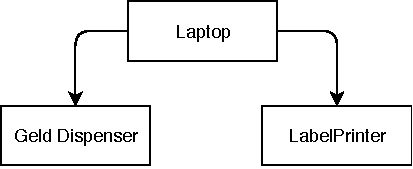
\includegraphics[height=0.9in]{netwerk_diagram.pdf}
        \caption{Netwerk Diagram}
        \label{fig: Netwerk Diagram}
\end{figure}

Hieronder is in pseudocode te zien welke opdrachten de laptop kan versturen naar de verbonden apparaten 
\lstinputlisting{communicatie.pseudo}


\newpage
\subsection{Bonnen}

\begin{figure}
        \centering
        
\includegraphics[height=2.0in]{obama_bon.pdf}
       \caption{Bon ontwerp}
       \label{fig: Bon ontwerp}
\end{figure}

Voor het uitgeven van bonnen hebben wij een labelprinter gebruikt.
In figuur \ref{fig: Bon ontwerp} is de bon te zien die de printer uitprint.
Hieronder is een link naar de sourcecode.

\vspace{1mm}\

\Mundus~\href{https://github.com/Gewad/Project4Bankalicious/tree/master/bonnetjesPrinten}{Code labelprinter}

\paragraph{Pseudocode uitleg}\ 

\lstinputlisting{Printerclass.pseudo}

\newpage

\subsection{Materiaal}

Er zijn hier een paar opties.
We kunnen bijvoorbeeld onderdelen 3d printen, maar dat zou erg duur zijn.
Het meest voor de hand liggende materiaal is triplex hout.
Dit is een redelijk goedkoop, en makkelijk verkrijgbaar materiaal.
Wij kunnen dit in het \emph{Tesla Lab} ophalen en daar direct uitsnijden.

\section{Ontwerp \& realisatie}

\subsection{Bouwtekening ATM}

Kijk wij kunnen tekenen!

\subsection{Toepassen kwaliteitseisen}

In deze paragraaf worden de de kwaliteids eisen die we eerder hebben opgesteld vergeleken met het eindproduct.


\paragraph{De code moet leesbaar zijn voor iedereen dus ook voor mensen die het niet geschreven hebben. Het doel is dat al onze ouders ook kunnen begrijpen wat er staat, een onderdeel hier van is commends.}
We denken niet dat onze ouders de code kunnen begrijpen, de code is wel lees en begrijpbaar door anderen mensen met programeer kennis. We hebben wel overal netjes code ingesprongen.
\paragraph{De code moet zo efficiënt mogelijk zijn.}

De code is redelijk efficent, er zit alleen wel een while(true), daarom is het programma vrij zwaar op het systeem. Een mogelijkheid om de code te verbeteren is het vervangen van wile loop's door interupts.
\paragraph{Variabele moeten een goede en duidelijk naam hebben en een vaste structuur volgen, namen van klasse beginnen met een Hoofdletter, namen van andere variabelen beginnen met een kleine letter.}
Dit hebben we goed gedaan.
	\paragraph{Als een variabele bestaat uit twee woorden begint het tweede woord met een Hoofdletter. Aka camelcase bv. camelCase.}
Dit hebben we ook goed gedaan.
	\paragraph{Splits zoveel mogelijk code op in classes en methodes. Stop bijbehorende code in een pakkage.}
We hebben redelijk veel verschillende classes en methodes, dit had meer kunnen zijn maar is over het algemeen goed. We hebben geen pakkage's gebruikt.
	\paragraph{Maak eerst een klasse diagram voor dat je gaat programmeren.}
Het grootste gedeelte van de code was al klaar voordat we met dit project begonnen dit is daarom onrelevand.
	\paragraph{In bestandsnamen mogen geen * worden gebruik dit vind Windows namelijk niet leuk.}
We hebben een * gebruikt in bestands namen.
\subsubsection{Product eisen}

	\paragraph{De geldautomaat moet  biljetten van tenminste vier verschillende waarden uit kunnen geven}
Dat kan
	\paragraph{De gebruiker kan niet, zonder een pin-opdracht te geven, geld uit de automaat halen}
Het is niet mogelijk om geld uit de automaat te halen zonder pin opdracht.
	\paragraph{De geldautomaat geeft altijd het juiste bedrag}
Meestal geeft de automaat het juiste bedrag, er zijn allen momenten dat er per ongeluk een extra biljet uit komt.
	\paragraph{De geldautomaat geeft alleen geld als het saldo toereikend is}
De automaat cheked eerst het saldo voordat hij geld uitgeeft.
	\paragraph{De gebruiker kan zelf selecteren welke biljetten hij/zij wil ontvangen}
Dit kan, mits er genoeg biljetten in de automaat zitten.
	\paragraph{De gebruiker kan geen biljetten kiezen die niet aanwezig zijn in de geldautomaat}
De automaat houdt bij hoeveel biljetten er nog in de automaat zitten.
	\paragraph{De geldautomaat is robuust (kan zelfstandig staan en valt niet om/uit elkaar tijdens gebruik)}
De automaat is stefig genoeg om te blijven staan en niet uit elkaar te vallen, als er geweld word gebruikt gaat hij wel kapot.
	\paragraph{De biljetten in de geldautomaat mogen maximaal de dikte van een speelkaart hebben}
We gebruiken speelkarten als biljetten, die zijn dus niet te dik.
	\paragraph{Na het pinnen wordt er een bon geprint met een bonprinter. Op deze bon staat in ieder geval hoeveel geld er is opgenomen en bij welke (lokale of individuele) bank dit is gebeurd}\
De bonnetjes printen, op de bonnetjes staat ht loge van de bank, de naam van de klant, het opgenomen bedrag, bij welke automaat de pintransactie is gedaan, de datum en de tijd.
	\paragraph{Er moet encryptie gebruikt worden tussen de geld automaat en de server en tussen de arduino en de computer.}
Dit hebben we niet gedaan.

\subsubsection{Eindgebruiker eisen}

	\paragraph{Een mooie en overzichtelijke gui voor de pin automaat, het moet de oma test kunnen doorstaan (als er tijd is gaan we het echt proberen).}
We hebben de oma test niet geprobeerd maar vinden de gui zelf erg duidelijk.
	\paragraph{Het moet niet zomaar uitvallen.}
Tenzij de gebreuker het actief kapot maakt blijft het werken.
	\paragraph{De pin automaat moet duidelijk terug communiceren wat de automaat verwacht.}
Dit is over het algemeen goed maar kan op sommige momenten nog net iets beter.
	\paragraph{Als er geld afgeschreven wordt komt er het zelfde bedrag uit de automaat.}
Dit gaat meestal goed, soms komt er allen iets te veel geld uit.
	\paragraph{Als er lange tijd niks gebeurd wordt de gebruiker automoties uitgelogd.}
Dit gebeurt niet.

\subsubsection{Git eisen}

	\paragraph{Niet op de master werken. Je werkt altijd op een eigen kopie van de test branch.}
Ja dit hebben we allemaal gedaan.
	\paragraph{Gelieve geen word bestanden te uploaden zonder ook een pdf te uploaden.}
We hebben alle word bestanden ook geupload als .pdg.
	\paragraph{Commits moeten duidelijk beschrijven wat er is aangepast. Liever een paar woorden te veel dan te weinig.}
De meeste commits zij vrij duidelijk, sommige hadden beter gekund.
	\paragraph{De repo van project 4 is geen zandbak om Git te testen.}
We hebben de project 4 repo niet gebruikt als zandbak.
	\paragraph{Directories zijn met kleine letters en underscores, en hebben een duidelijke naam.}
Alle directories voldoen aan deze eisen behalve die van Floor.
	\paragraph{Alle benamingen en commits moeten in het Nederlands.}
Het grootste deel van de commits is voledig in het nederlands, sommige computer termen zijn wel in het engels.


\subsubsection{Code eisen}


\subsection{Testen}

\textbf{Aron moet dit doen}
Tijdens het testen...
Dit dat blijkt kut...
Dit dat zo gefixed...

\end{document}
